\documentclass[11pt]{article}

%====================== PACKAGES ======================

\usepackage[utf8]{inputenc}
\usepackage[french]{babel}
\usepackage{natbib}
\usepackage{url}
\usepackage{amsmath}
\usepackage{graphicx}
\usepackage{parskip}
\usepackage{fancyhdr}
\usepackage{hyperref}
\usepackage{tabularx}
\usepackage{vmargin}
\usepackage{setspace}
\usepackage{wrapfig}
\usepackage{filecontents}
\usepackage{tikzsymbols}
\usepackage{metre}
\usepackage{minted}
\usepackage{tabularx}
\usepackage{longtable}
\usepackage{tikz}
\usepackage[nottoc, notlof, notlot]{tocbibind}

%====================== INFORMATION ET REGLES ======================

\setmarginsrb{2.5 cm}{1.5 cm}{2.5 cm}{1.5 cm}{1 cm}{1 cm}{1 cm}{1.5 cm}
\renewcommand{\baselinestretch}{1.3} 

\title{Stage de fin d'étude - Etude de sécurité d'un contrôleur SDN : ONOS}                             
\author{Julien Schoumacher}
\date{\today}

\hypersetup{
pdfauthor = {\@author},
pdftitle = {\@title},
pdfsubject = {Mémoire de stage d'ingénieur},
pdfkeywords = {SDN, ONOS, sécurité},
pdfstartview = {FitH}}

\graphicspath{ {images/} }

\newcommand*\circledred[1]{\tikz[baseline=(char.base)]{\node[shape=circle,fill=red,draw,inner sep=2pt] (char) {#1};}}
\newcommand*\circledorange[1]{\tikz[baseline=(char.base)]{\node[shape=circle,fill=orange,draw,inner sep=2pt] (char) {#1};}}
\newcommand*\circledgreen[1]{\tikz[baseline=(char.base)]{\node[shape=circle,fill=green,draw,inner sep=2pt] (char) {#1};}}
\newcommand*\circledcyan[1]{\tikz[baseline=(char.base)]{\node[shape=circle,fill=cyan,draw,inner sep=2pt] (char) {#1};}}
\newcommand*\circled[1]{\tikz[baseline=(char.base)]{\node[shape=circle,draw,inner sep=2pt] (char) {#1};}}

%====================== Bibliographie ======================

\begin{filecontents}{references.bib}

@misc{of_def,
  author = {Open Networking Foundation},
  title = {{Software-Defined Networking (SDN) Definition}},
  howpublished = "\url{https://www.opennetworking.org/sdn-resources/sdn-definition}",
}

@misc{indirection,
  title = {{Fundamental theorem of software engineering}},
  howpublished = "\url{https://en.wikipedia.org/wiki/Fundamental_theorem_of_software_engineering}",
}

@article{rapport_maxence,
  title = {Mémoire de stage : Étude d’OpenFlow dans le contexte de la sécurité},
  author = {Maxence Tury}
}

@misc{histoire,
  title = {A Survey of Software-De ned Networking:  Past, Present, and Future of Programmable Networks},
  author = {{Bruno Nunes Astuto, Marc Mendonça, Xuan Nam Nguyen, Katia Obraczka, Thierry Turletti}},
  howpublished = "\url{https://hal.inria.fr/hal-00825087/file/hal_final.pdf}"
}

@misc{openflow_google,
  title = {Openflow at Google},
  author = {Hoelzle Tue},
  howpublished = "\url{http://opennetsummit.org/archives/apr12/hoelzle-tue-openflow.pdf}"
}

@misc{OF_10,
  title = {Spécification Openflow 1.0},
  howpublished = "\url{http://archive.openflow.org/documents/openflow-spec-v1.0.0.pdf}"
}

@misc{OF_13,
  title = {Spécification Openflow 1.3},
  howpublished = "\url{https://www.opennetworking.org/images/stories/downloads/sdn-resources/onf-specifications/openflow/openflow-spec-v1.3.0.pdf}"
}

@misc{OF_15,
  title = {Spécification Openflow 1.5},
  howpublished = "\url{https://www.opennetworking.org/images/stories/downloads/sdn-resources/onf-specifications/openflow/openflow-switch-v1.5.0.noipr.pdf}"
}

@misc{Vulns,
  author = {{K. Benton, L.J. Camp, and C. Small}},
  title = {OpenFlow Vulnerability Assessment},
  howpublished = "\url{http://conferences.sigcomm.org/sigcomm/2012/paper/hotsdn/p121.pdf}"
}

@misc{Security_analysis_controllers,
  title = {Security Analysis of OpenDayLight, ONOS, RoseMary and RYU SDN Controllers},
  author = {{Ramachandra Kamath Arbettu, Kpatcha Bayarou, Frank Weber}},
  howpublished = "\url{http://publica.fraunhofer.de/eprints/urn_nbn_de_0011-n-4046948.pdf}"
}

@misc{Security_analysis_protocols,
  title = {Security Analysis of Software Defined Networking Protocols—OpenFlow, OF-Config and OVSDB},
  author = {{Markus Brandt, Rahamatullah Khondoker, Kpatcha Bayarou, Frank Weber}},
  howpublished = "\url{http://publica.fraunhofer.de/eprints/urn_nbn_de_0011-n-3238618.pdf}"
}

@misc{anomaly_detection,
  title = {Combining OpenFlow and sFlow for an effective and scalable anomaly detection and mitigation mechanism on SDN environments},
  author = {{K. Giotis, C. Argyropoulos, G. Androulidakis, D. Kalogeras, V. Maglaris}},
  howpublished = "\url{http://www.sciencedirect.com/science/article/pii/S1389128613004003}"
}

@misc{debugger,
  title = {Where is the Debugger for my Software-Defined Network?},
  author = {{Nikhil Handigol, Brandon Heller, Vimalkumar Jeyakumar}},
  howpublished = "\url{https://users.ece.cmu.edu/~vsekar/Teaching/Fall14/18859K/papers/ndb.pdf}"
}

@misc{sdn_security,
  author = {David Jorm},
  title = {SDN and Security},
  howpublished = "\url{http://onosproject.org/2015/04/03/sdn-and-security-david-jorm/}"
}

@misc{poisoning,
  title = {Poisoning Network Visibility in Software-Defined Networks: New Attacks and Countermeasures},
  author = {{Sungmin Hong, Lei Xu, Haopei Wang, Guofei Gu}},
  howpublished = "\url{http://www.internetsociety.org/sites/default/files/10_4_2.pdf}"
}

@misc{towards,
  title = {Towards Secure and Dependable Software-Defined Networks},
  author = {{Diego Kreutz, Fernando M. V. Ramos, Paulo Verissimo}},
  howpublished = "\url{https://www.ietf.org/proceedings/87/slides/slides-87-sdnrg-2.pdf}"
}

@misc{security_mode,
  author = {Changhoon Yoon},
  title = {Security-Mode ONOS},
  howpublished = "\url{http://events.linuxfoundation.org/sites/events/files/slides/smonos_ons2016.pdf}"
}

@misc{inter_clustering,
  author = {{bubakar Siddique Muqaddas, Andrea Bianco, Paolo Giaccone, Guido Maier}},
  title = {Inter-controller Traffic in ONOS Clusters for SDN Networks},
  howpublished = "\url{http://www.telematica.polito.it/~giaccone/papers/icc16-onos.pdf}"
}

@misc{next_gen,
  author = {Changhoon Yoon, Seungsoo Lee},
  title = {Attacking SDN Infrastructure Are We Ready For The Next Gen Networking ?},
  howpublished = "\url{https://www.blackhat.com/docs/us-16/materials/us-16-Yoon-Attacking-SDN-Infrastructure-Are-We-Ready-For-The-Next-Gen-Networking.pdf}"
}

@misc{ONOS_REST,
  title = {The Smaller, the Shrewder: A Simple Malicious Application Can Kill an Entire SDN Environment},
  author = {{Seungsoo Lee, Changhoon Yoon, Seungwon Shin}},
  howpublished = "\url{http://nss.kaist.ac.kr/wp-content/uploads/2016/05/p23-lee.compressed.pdf}"
}

@misc{Wireshark,
  title = {OpenFlow for Wireshark},
  howpublished = "\url{http://wiki.wireshark.org/OpenFlow}"
}

\end{filecontents}


%======================== DEBUT DU DOCUMENT ========================

\pagestyle{fancy}
\fancyhf{}
\fancyhead[C]{~\\}
\fancyfoot[C]{\thepage}

\begin{document}



%page de garde
\begin{titlepage}
	\newcolumntype{s}{>{\hsize=.25\hsize}X}
	\begin{tabularx}{\textwidth}{lsrl}
		
\includegraphics[width=0.2\textwidth]{TelecomParisTech_logo_200_01.png}
		&
    	\shortstack{\huge{Télécom} \\ \huge{ParisTech}}
    	&
		
\includegraphics[width=0.2\textwidth]{Logo_SP.jpg}
		&
		\shortstack{\huge{Télécom} \\ \huge{SudParis}}
	\end{tabularx}

    \begin{center}
        \vspace*{1cm}
        
        \Huge
       	~\\
       	~\\
       	~\\
        \textbf{Mémoire de stage}
        
        \vspace{0.5cm}
        \LARGE
        Sécurité d'un contrôleur SDN : ONOS\\
        ~\\
        
        \vspace{1.5cm}
        
        \textbf{Julien Schoumacher}
        
        \vfill
       
        \begin{flushleft}
       		 Diplôme préparé : Ingénieur\\
        	 Stage effectué du 20 juillet 2016 au 20 janvier 2017 à Télécom SudParis sous la direction de Grégory Blanc
        \end{flushleft}
        \vspace{0.3cm}
        
    \end{center}
\end{titlepage}

%======================== Remerciements ========================
\newpage
{\large ~\\}
\section*{\Huge{Remerciements}}
~\\
{\Large~~~~~~~
Avant d'entamer la lecture de ce rapport, je tiens avant tout à remercier toute l'équipe du département RST (Réseaux et Services des Télécommuni-cations) de Télécom SudParis qui m'a si bien accueilli durant ce stage. Je remercie également mon encadrant côté Télécom ParisTech Rida Khatoun, m'ayant mis en relation avec le maître de conférences Gregory Blanc qui m'a encadré avec bienveillance pendant toute la durée du stage. Enfin, toutes les autres personnes que j'ai pu cottoyer plus ou moins longtemps à l'occasion d'évènements ponctuels comme la conférence RAID qui s'est tenue en septembre.}
\phantomsection

%======================== Table des matières ========================
\newpage
\tableofcontents


\newpage
\fancyhead[L]{1- Réseau SDN}
\section{Réseau SDN (Software Defined Network)}
	\subsection{Motivation}
		On ne peut pas entamer cette étude portant en partie sur les réseaux SDN sans oublier de mentionner quelques éléments difficilement contestables sur les réseaux actuels \footnote{\label{of_def}Aussi résumé dans \url{https://www.opennetworking.org/sdn-resources/sdn-definition}} :

\begin{itemize}

\item La demande ne cesse de croître : on observe un accroissement considérable des enjeux liés au traitement de masse importante de données, de l'utilisation de services cloud, du trafic mobile et peut être bientôt de l'utilisation d'objets connectés. Or tous ces éléments présentent le point commun de communiquer avec de nombreuses entités situées sur des réseaux potentiellement éloignés. Cela mobilise donc un trafic réseau intense.

\item Les technologies actuelles pour soutenir cette demande énorme sont capables de fournir un débit titanesque : que l'on considère des technologies sans fil ou non, au coeur des réseaux tant au niveau des terminaux des utilisateurs, on atteint aujourd'hui des débits théoriques de l'ordre du Gigabit par seconde pour l'utilisateur. Tout cela sans que l'on ait vraiment conscience des conditions que cela requiert.

\item Les méthodes d'accès sont aujourd'hui bien différentes. Précédemment le modèle client/ serveur était largement employé, avec dans le cas d'une entreprise, un réseau interne constitué de plusieurs LAN séparés, et connecté à internet de manière quasiment unique. Cela entraînant une configuration possiblement statique et donc aisée, les échanges se déroulant principalement sur un mode requête/réponse. Or la tendance, notamment à cause des deux premiers points, est à l'émergence de nouveaux modes d'accès plus horizontaux (avec d'avantage d'entités faisant circuler l'information au même niveau "hiérarchique"). Ce type de communication tient entre autres de la distribution plus éparse des données à travers le réseau due au grossissement de la taille des bases de données, à la duplication de celles-ci (mise en cache sur différents serveur à travers le monde pour permettre un accès plus rapide), à l'augmentation du trafic volumineux (vidéo, voix) et de nouveaux trafics (IoT, Bring Your Own Device, ...) même au sein de l'entreprise. Enfin, l'utilisation de plus en plus répandue de services cloud, avec ses implications au niveau de la virtualisation (que ce soit des applications, ou bien des bases de données), susceptible de changer en permanence la localisation des serveurs pour garantir une certaine flexibilité.

\end{itemize}

Or, le réseau principal global tel que nous le connaissons (la partie reposant sur TCP/IP en tout cas) a été conçu d'abord dans un but de fiabilité : chaque paquet doit être reçu, peu importe la route empruntée. L'architecture distribuée actuelle n'est donc pas bâtie pour assurer spécifiquement une extension aisée des services fournis, ni une qualité de service définie. Le routeur (et le réseau d'ailleurs) des années 1980 a donc été progressivement amélioré sur la base de ce paradigme initial, avec le plan de données et le plan de contrôle attachés aux mêmes équipements, configurés en partie manuellement. Tout s'est complexifié également : nouveaux protocoles, ajouts d'équipements spécifiques (capables de répartir la charge réseau, de filtrer les paquets, de prévenir de certaines tentatives d'attaque, etc ...), ...\\
Certains éléments de réflexion peuvent éventuellement nous mettre sur la voie d'une complexité qui, à défaut d'être exponentielle, l'est d'avantage que simplement linéaire (c'est du moins une conviction personnelle non vérifiée) :

\begin{itemize}
\item Plus il y a d'éléments statiques dans un réseau, et plus la propagation des modifications d'ensemble est coûteuse (puisqu'il faut penser à chaque impact sur les parties statiques et modifier un à un chaque équipement).
\item Si un problème survient, il est difficile d'avoir une vue globale de ce qui se passe puisqu'à moins de disposer d'équipements spéciaux aucune vue globale du réseau n'est accessible : il faut vérifier (potentiellement) que chaque élément se comporte correctement et est bien configuré.
\item Les interfaces entre switchs, routeurs et autres éléments peuvent varier selon le constructeur, et le logiciel sur les équipements est souvent propriétaire et complexe, surtout dans le cas de gros réseaux hétérogènes, ce qui ne facilite pas forcément la bonne marche de l'ensemble.
\end{itemize}

De nombreux problèmes se résolvent avec un niveau d'abstraction supplémentaire \footnote{\label{indirection}\url{https://en.wikipedia.org/wiki/Fundamental_theorem_of_software_engineering}}. Si le dévelop-pement de systèmes de plus en plus complexes s'est fait de manière très rapide sur PC, c'est d'abord grâce à la première couche d'abstraction qu'ont constitué les instructions assembleur, puis à la seconde qu'a été le système d'exploitation. Certaines personnes ont eu l'idée, au lieu de considérer le réseau comme un élément périphérique, de le voir comme un processeur capable d'exécuter des instructions basiques, fournissant de fait un service plus facilement adaptable. C'est sur ce principe que repose le Software Defined Network (SDN). Avec une couche d'abstraction supplémentaire que constitue le protocole choisi pour véhiculer le flot d'instructions (OpenFlow dans notre cas, mais il y en a d'autres que nous évoquerons succintement plus tard), et un système d'exploitation spécifique (Network Operating System, NOS), l'idée est de découpler les différents chemins qu'empruntent les données et le plan de contrôle, à la manière d'un système d'exploitation qui sépare le code d'un programme et les données qu'il utilise.
		~\\
	\subsection{Concepts}
		La dernière analogie (avec un ordinateur) peut être poursuivie de la manière suivante. Sur un PC classique, on crée et utilise des applications qui reposent sur un système d'exploitation responsable des éléments matériels. De manière similaire, le modèle SDN permet la création d'applications "réseau" sans se soucier de la traduction des décisions de routage des paquets au niveau applicatif en routage au niveau des interfaces physiques.\\

Pour réaliser cela, il est nécessaire, puisqu'un réseau est constitué d'entités physiquement séparées, de disposer d'un protocole de communication standard entre celles-ci. Mais ça n'est pas suffisant : des instructions de routage doivent également être distribuées. Cela n'est possible que si il existe un cerveau central qui coordonne les opérations (il n'existe pas vraiment d'intelligence collective à ce jour). C'est le rôle du contrôleur SDN. On déporte ainsi l'intelligence humaine déployée dans la configuration de tous les éléments du réseau vers un seul (même si il peut être dupliqué).\\

\begin{figure}[h]
  	\centering
  	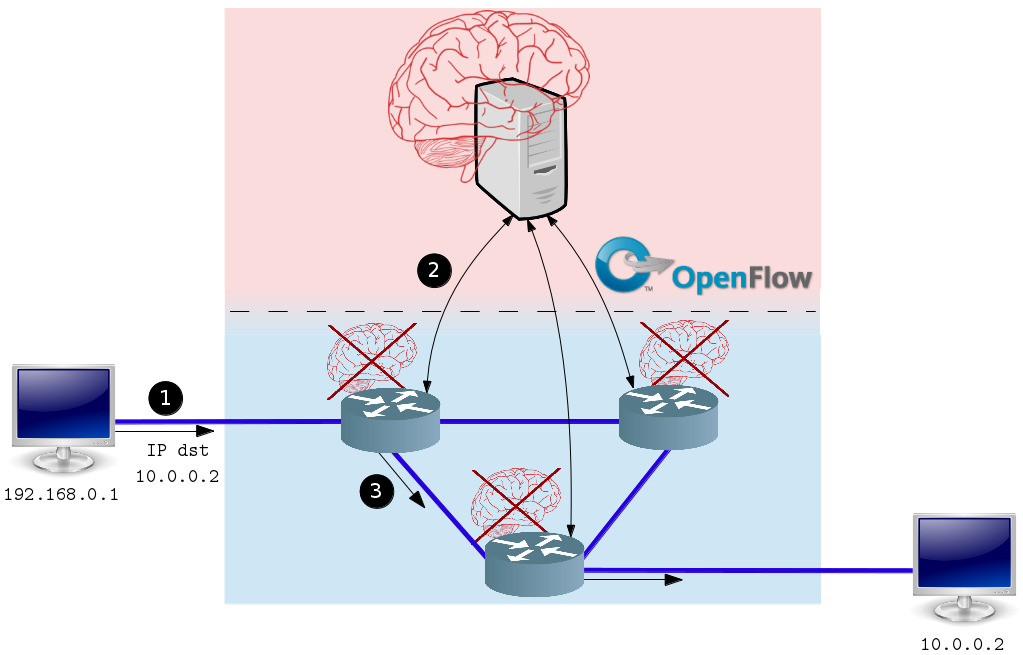
\includegraphics[width=0.8\textwidth]{openflow.png}
  	\caption[Caption for LOF]{Réseau SDN : "l'intelligence" est déportée vers le contôleur \footnotemark}
\end{figure}

\footnotetext{\label{rapport_maxence} Schéma extrait du mémoire "Étude d’OpenFlow dans le contexte de la sécurité" de Maxence Tury}

\begin{figure}[h]
  	\centering
  	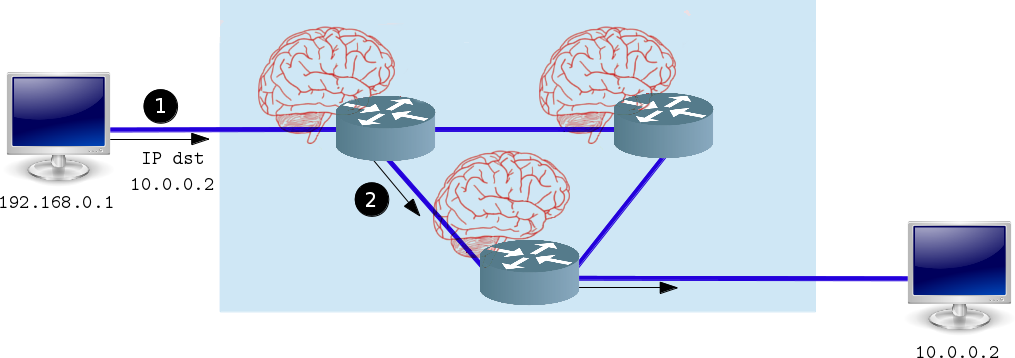
\includegraphics[width=0.85\textwidth]{routage_normal.png}
  	\caption{Réseau classique : chaque routeur contient une partie de la logique de contrôle}
\end{figure}

Les avantages de cette architecture sont multiples :
\begin{itemize}
\item D'abord cela réduit grandement la complexité de configuration manuelle et le risque d'erreur (si le système d'exploitation réseau est fiable).
\item Cela facilite donc énormément le développement d'applications réseau complexes, puisque la tâche peut être quasiment séparée de sa réalisation physique.
\item Les routes optimales sont plus facilement calculables qu'au sein d'un réseau classique : un seul élément gère les différentes distances et métriques qui peuvent changer selon le trafic, et être modifiées à la volée par des applications spécifiques.
\item La gestion du réseau devient plus simple, les évènements importants (perte d'un lien, dysfonctionnement, ralentissement ...) peuvent être remarqués rapidement, la réaction pouvant être automatique et quasiment instantanée.
\item Les coûts matériels sont globalement diminués puisqu'un switch programmable Openflow peut n'implémenter que le protocole en question pour être fonctionnel (le reste pouvant être pris en charge logiciellement au niveau du contrôleur). Il est également possible de migrer partiellement vers une architecture SDN en utilisant des switchs hybrides.
\end{itemize}

Pour résumer, beaucoup plus de flexibilité est permise par cette approche, économisant temps et matériel. Évidemment, l'idée n'est pas nouvelle, mais n'a pas que des avantages. Notamment : la sécurité du contrôleur devient un point brûlant, puisque toute la gestion du réseau repose sur lui.
		~\\
	\subsection{Historique}
		L'idée d'une séparation entre plan de données et plan de contrôle n'est pas nouvelle, et cette partie se propose de retracer succinctement diverses voies qui ont abouti à l'adoption assez univoque du protocole OpenFlow comme interface entre les deux. Pour obtenir un état de l'art détaillé et complet, il est possible de consulter les articles "A Survey of Software-Defined Networking: Past, Present, and Future of Programmable Networks"\footnote{\label{histoire}\url{https://hal.inria.fr/hal-00825087/file/hal_final.pdf}} (2014) et "Software-Defined Networking: A Comprehensive Survey"\footnote{\url{http://www.hit.bme.hu/~jakab/edu/litr/SDN/Long_Survey_06994333.pdf}} (2015).\\

Assez tôt est apparue l'idée de rendre les switchs programmables : dès 1990, le groupe Open Signaling propose un protocole de contrôle de switchs à distance appelé GSMP (General Switch
Management  Protocol). Si les possibilités restent assez limitées (essentiellement gestion des ports, redirection de trafic sur des ports contrôlés, et obtention de statistiques), cela permet néanmoins un accès au matériel plus aisé.

D'autres approches sont testées dans la même période : l'initiative Active Networking propose quant à elle un mécanisme de propagation de code que l'équipement réseau exécute lorsqu'il reçoit les paquets encapsulant le code (même si cela pose un gros problème en matière de sécurité).

Le groupe DCAN (Devolved Control of ATM Networks) propose une approche qui se rapproche très fortement du paradigme SDN : ils développent un protocole minimaliste entre une entité spécialisée (le contrôleur) et autres équipements et mettent en place une gestion semi-automatique du réseau pour partitionner les ressources disponibles (ils rajoutent donc la possibilité de programmer le contrôleur).\\

Le projet 4D \footnote{\url{http://www.cs.cmu.edu/~4D/}} initié en 2004, présente une formalisation du concept : on cherche à obtenir la possibilité de prendre des décisions réseau en dehors des équipements physiques, ce qui nécessite l'obtention d'un maximum d'informations à la fois sur la composition physique du réseau, et sur les liens qui existent entre chaque élément. L'incorporation des services globaux que sont la découverte de la topologie et la dissémination d'informations sur l'état général du réseau associée à la possibilité d'agir sur le réseau est ce qui a inspiré l'idée de système d'exploitation réseau, qu'implémentent aujourd'hui les contrôleurs SDN.\\

On peut encore citer NETCONF et Ethane (2006), le premier pouvant être vu comme une extension de SNMP, le second comme un ancêtre immédiat d'OpenFlow. Même si la finalité d'Ethane était plus axée sur une gestion des identités (vérification des droits d'un paquet à circuler sur le réseau entre autres) que sur une gestion générale du réseau, c'est un protocole entre switch programmable et contrôleur encapsulant des actions à effectuer sur des paquets reçus au niveau du switch (ces actions étant essentiellement limitées à de la redirection/suppression).\\

OpenFlow a quant à lui précédé l'apparition du terme SDN lors d'expérimentations à Stanford vers 2010 (la première spécification d'OpenFlow pour la production (1.0.0), a été publiée début 2010).
		~\\
	\subsection{Exemples d'applications}
		En 2011, l'Open Networking Foundation (ONF) est créée. Regroupant des gros acteurs comme Google, Yahoo, Facebook, Verizon, Microsoft ou encore Deutsche Telekom, c'est l'organisme principal qui encourage l'adoption de la technologie SDN, en publiant régulièrement de nouvelles spécifications Openflow.\\

Google, en 2012, présente, pour la première fois, une architecture SDN pour ses datacenters, utilisant Openflow sur des switchs conçus par eux-mêmes (étant pionniers, leur position étant qu'ils auraient utilisé des switchs existants si ceux-ci implémentaient toutes les fonctionnalités Openflow leur étant nécessaires). Grâce à ce nouveau paradigme, Google affirme (en 2012) obtenir des performances dix fois supérieures en terme de débit, et surtout utiliser 100\%\footnote{\url{http://www.networkworld.com/article/2189197/lan-wan/google-s-software-defined-openflow-backbone-drives-wan-links-to-100--utilization.html}} de leurs lignes (contrairement aux 30 à 40\% en vigueur dans l'industrie, notamment pour garantir un service même en cas de nombreuses pannes, ce qui n'est plus nécessaire avec un réseau SDN qui adapte automatiquement le routage pour pallier aux problèmes).\\

Microsoft semble également s'être intéressé au SDN pour son service "Azure" depuis quelques années maintenant \footnote{\url{http://www.networkworld.com/article/2937396/cloud-computing/microsoft-needs-sdn-for-azure-cloud.html}}, et de manière générale toutes les figures de proue de l'industrie  numérique (celles qui disposent de nombreux serveurs et gèrent des flux énormes et grandissants de données comme Amazon, AT\&T, Facebook, ...) se sont plus ou moins annoncées investies dans le processus, possiblement avec leur propre protocole SDN. Si des grosses entreprises ont annoncé l'utilisation de ce type de réseau, les données précises concernant les performances obtenues sont difficilement accessibles, ce qui rend compliquée l'évaluation des avantages réels de SDN.\\

Par ailleurs, les switchs compatibles Openflow, ou les switchs Openflow seuls, que fournissent (depuis 2011 environ) certaines entreprises majeures du domaine comme Brocade, HP, IBM, Juniper ou encore NEC, Pronto ou Pica8, manquent encore parfois de maturité (RFC parfois interprétée différemment, vulnérabilités spécifiques, ...). L'évolution des versions Openflow est également parfois difficile à suivre (la spécification de la version 1.0.0 (fin 2009) fait 42 pages\footnote{\label{OF_10}\url{http://archive.openflow.org/documents/openflow-spec-v1.0.0.pdf}}, celle de la dernière version stable (1.5.0, fin 2014) en fait 277 \footnote{\label{OF_15}\url{https://www.opennetworking.org/images/stories/downloads/sdn-resources/onf-specifications/openflow/openflow-switch-v1.5.0.noipr.pdf}}). Or l'industrie dans ce domaine présente une certaine inertie (peu sont les compagnie qui proposent des switchs compatibles avec la dernière version d'Openflow, certaines vendant encore des switchs Openflow 1.0).\\

Les applications semblent donc d'un premier abord limitées aux datacenters (beaucoup de données à traiter, grande variabilité de la topologie (les machines virtuelles changent souvent d'emplacement/adresse)). En réalité, SDN peut être utilisé de manière effective dans plusieurs cas :

\begin{list}{$\Asteriscus$}{}
\item Réseaux d'entreprises/universités : dans le cas de nombreux équipements/protocoles différents utilisés, SDN permet théoriquement de faciliter le déploiement de politiques réseau complexes.
\item Réseaux optiques : faciliter la transition, la gestion et l'incorporation des réseaux optiques au sein du réseau actuel.
\item Infrastructure based WAN (réservé aux entreprises disposant de nombreux serveurs à travers le monde) : à la manière de Google, un moyen de connecter de grosses entités en évitant les goulots d'étranglement. Egalement un moyen envisageable pour un utilisateur de se connecter depuis n'importe quel endroit en disposant des services auxquels il souscrit.
\item Infrastructure personnelle, petites entreprises : surveiller le trafic et alerter l'administrateur local ou le fournisseur internet en cas de détection d'activité réseau suspecte (utile notamment dans le cadre de l'IoT).\\
\end{list}

Au final, une technologie pouvant sembler prometteuse, mais demeurant assez peu utilisée pour plusieurs raisons. Nous allons en étudier deux d'entre elles par la suite : la sécurité générale du réseau, et l'importance capitale du contrôleur qui devient quasiment l'unique clé de voûte du système.
\newpage
\fancyhead[L]{2- Cadre de l'étude}
\section{Cadre de l'étude}
	\subsection{Problématique et objectifs}
		Mon stage, dont le sujet n'était pas complètement fixé au départ, a pris la tournure suivante : d'abord une étude des réseaux SDN (ne connaissant pas le domaine), puis début d'expérimentations sur le protocole Openflow, avec Scapy et Wireshark. Ensuite, constitution d'un rapide état de l'art en matière d'attaques (générales) sur les réseaux SDN. Puis, l'orientation s'est faite sur l'étude plus précise d'un contrôleur SDN particulier (ONOS), avec la conception de scénarios d'attaque, suivie de leur réalisation.\\
Comme on l'a dit au-dessus, le contrôleur SDN est le point névralgique de toute l'infrastructure. Si on le compromet d'une manière où d'une autre, les conséquences peuvent être désastreuses. L'étude a donc eu pour but de déterminer les principaux vecteurs d'attaque envisageables dans ce genre de réseau, principalement concernant le contrôleur ONOS (principalement, parce qu'il  est possible d'appliquer une majorité des attaques sur d'autres contrôleurs, même si cela n'a pas été expérimentalement vérifié).\\
Pour résumer, un audit (se voulant le plus exhaustif possible, même si il est impossible de couvrir l'ensemble des vulnérabilités d'un tel élément logiciel) a été réalisé. Cet audit a été conçu informellement à partir de la méthode STRIDE\footnote{STRIDE = Spoofing, Tampering, Repudiation, Info disclosure, Denial of service, privilege Escalation, qui respectivement permettent de vérifier les propriétés d'authentification, d'intégrité, de non-répudiation, de confidentialité, de disponibilité et d'autorisation} (utilisée par microsoft à la base, cette manière de modéliser les menaces dans le domaine de la sécurité s’est beaucoup répandue). Certains scénarios ont été expérimentés pour prouver la faisabilité d'attaques précises (donc sous certaines hypothèses qui sont décrites). D'autres faiblesses sont également détaillées dans leur aspect théorique sur la base de sources externes. Bien que n'ayant pas eu accès à une situation réelle de déploiement SDN, j'essaierai de donner une conclusion pas trop biaisée aux tests effectués, et formulerai quelques recommandations et remarques.
	\subsection{Architecture d'un réseau SDN}
		Avant toute chose, il est nécessaire de détailler la façon dont un réseau SDN fonctionne, afin que les attaques qui seront évoquées plus tard puissent être bien comprises. Pour cela, on insistera particulièrement sur la description du protocole Openflow, mais aussi sur celle de l'objet de notre étude, ONOS.
		\subsubsection{Openflow}
			Openflow est un des protocoles qui permet de séparer le plan de données et le plan de contrôle (protocole majoritairement utilisé à l'heure actuelle, étant non propriétaire et porté par l'ONF). Pour l'utiliser, il est nécessaire de disposer de switchs compatibles, c'est à dire des switchs capables de gérer des paquets Openflow. Ainsi, les décisions prises au niveau du contrôleur sont transmises aux switchs concernés par le biais de ce protocole. Pour que l'abstraction de la gestion du réseau soit intéressante, le protocole permet aux switchs une gestion assez fine des paquets reçus à leur niveau, et ce jusqu'au niveau 4 (pour TCP comme on va le voir après). C'est le principal élément de ce qu'on appelle l'interface sud d'un réseau SDN (interface entre contrôleur et entités matérielles) :
\begin{figure}[h]
  	\centering
  	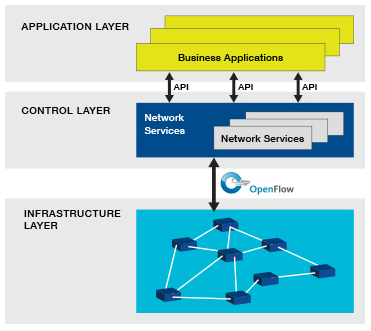
\includegraphics[width=0.45\textwidth]{interfaces.jpg}
  	\caption{Différentes interfaces, Openflow = interface sud}
\end{figure}

Chaque switch (qu'il soit compatible Openflow ou virtuel) consiste en plusieurs tables de flux et une table de groupe (non présente en version 1.0), ainsi qu'un (ou plusieurs) canal(aux) vers le(s) contrôleur(s) (sécurisé(s) via TLS obligatoire en version 1.0 mais obligation supprimée dès la version 1.1 pour des raisons de facilité de déploiement). La description du fonctionnement qui suit est celle de la version 1.3 du protocole (ça n'est donc ni la dernière version, ni la première, mais celle que j'ai principalement utilisée durant le stage, Wireshark la disséquant complètement).\\

La notion de flux est essentielle. Un flux est constitué de 3 parties :
\begin{list}{$\Asteriscus$}{}

\item La première une règle qui filtre les paquets : en fonction des attributs du paquet à l'entrée du switch (port d'entrée physique, adresse ethernet source, adresse ethernet destination, type de paquet, VLAN id, VLAN priority, adresse IP source, adresse IP destination, protocole IP, ToS IP, TCP port source, TCP port destination entre autres). Il est possible de générer des filtrages généraux avec l'utilisation de jokers (wildcard en anglais) sur les champs souhaités (par exemple, si on veut autoriser toutes les adresses ethernet source ayant pour adresse IP x.x.x.x, on pourra utiliser un joker sur le champ adresse ethernet source).

\item La seconde est un compteur qui permet de tenir à jour, si le switch le permet, des statistiques sur l'utilisation du flux.

\item La troisième est une action à appliquer en cas de correspondance du paquet : si le paquet remplit les conditions du filtre, plusieurs types de traitements sont possibles. Entre autres : envoyer le paquet au contrôleur, rediriger le paquet vers un port physique spécifique, vers une table de flux, vers tous les ports sauf le port d'entrée, vers les switchs voisins mis à jour par spanning tree, supprimer le paquet, ou encore modifier certains champs avant redirection, rediriger le paquet vers une queue. Bref, toutes les opérations envisageables sur un paquet. Certaines de ces actions doivent être prises en charge par les switchs Openflow pour que ceux-ci puissent être considérés comme tels. D'autres actions sont optionnelles (par exemple la redirection vers les switchs mis à jour par spanning tree).

\end{list}

Chaque nouveau flux ajouté au switch par le contrôleur l'est dans une table de flux spécifiée. Ainsi, plutôt que d'avoir à organiser relativement la priorité de chaque flux, des regroupements peuvent se faire par table pour factoriser certains traitements. Le switch parcourt chaque table de flux (en considérant le premier flux de chaque table) jusqu'à trouver un filtrage correct pour le paquet. A ce moment, le paquet parcourt et subit les traitements de chacun des flux dans la table trouvée (c'est la notion de pipeline Openflow) jusqu'à ce qu'une action de redirection soit trouvée. La redirection peut également être faite vers une table de flux de priorité inférieure (pour éviter qu'un paquet boucle indéfiniment).

\begin{figure}[h]
  	\centering
  	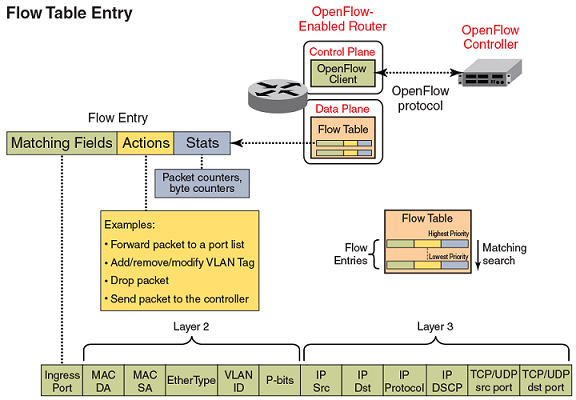
\includegraphics[width=0.9\textwidth]{brocade_flow.png}
  	\caption{Flux et table de flux}
\end{figure}

Basiquement, on peut résumer le protocole Openflow comme étant le protocole permettant :
\begin{list}{$\Asteriscus$}{}

\item de mettre à jour ces tables de flux : ajouts, ajouts partiels (par exemple ajouts de précisions à un flux avec joker), suppressions, modifications, etc ....  

\item d'obtenir des statistiques sur certains éléments (en Openflow 1.3, on peut accéder aux statistiques des flux, des tables, des ports, des queues, des groupes, ou encore du débit (pour la qualité de service)).

\item d'obtenir des informations sur les entités du réseau (nom de l'équipement, nom du fabricant, débit supporté ...)

\end{list}

C'est un protocole qui s'établit de manière classique sur une session TCP (éventuellement surmonté d'une session TLS), habituellement sur les ports 6633 ou 6653 (ce dernier étant maintenant alloué pour cet usage par l'IANA).\\
Il est constitué :

\begin{list}{$\Asteriscus$}{}

\item de messages symétriques (Hello, Echo), qui s'utilisent pour ou démarrer une session Openflow ou s'assurer que les deux parties sont encore connectées

\item de messages contrôleur vers switch (ressemblant à du requête/réponse), généralement les messages qui permettent au contrôleur d'obtenir des informations sur le switchs et de lui donner des ordres. Mais aussi, et c'est important, un message qui permet directement d'insérer du trafic dans le réseau. Ainsi, lorsque le switch envoie un paquet qu'il ne sait pas traiter au contrôleur, celui-ci peut le renvoyer au switch (après l'avoir traité et éventuellement modifié), ce qui évite de perdre le paquet \footnote{On appelle alors ce paquet OFPT\_PACKET\_OUT (selon la spécifiation) qu'on abrégera par la suite en PACKET\_OUT}.

\item de messages asynchrones émis par les switchs, qui sont par exemple susceptibles d'informer le contrôleur lorsqu'ils ont modifié, supprimé ou ajouté un flux, mais également lorsqu'un paquet ne correspond à aucun flux, qu'une erreur survient ou bien qu'un port physique change de configuration. Le message asynchrone le plus important est sûrement celui qui survient lorsque le switch doit envoyer le paquet au contrôleur \footnote{Paquet appelé OFPT\_PACKET\_IN (selon la spécifiation) qu'on abrégera par la suite en PACKET\_IN} (soit parce qu'une règle le demande explicitement, soit parce que le switch ne peut pas traiter le paquet et que la règle par défaut associée demande un envoi au contrôleur).

\end{list}

Ci-dessus une capture Openflow réalisée sous Wireshark.

La figure précédente provient de mes expérimentations, j'ai en effet été amené durant mon stage à créer une sorte de mini-switch virtuel très basique avec Scapy, ce qui m'a forcé à implémenter à la fois la pile TCP et la session Openflow . Même si par la suite cela m'a été peu utile pour réaliser mes scénarios d'attaque, cela m'a permis de bien comprendre le protocole Openflow.

Le lecteur désirant rentrer dans les détails techniques peut se référer à la spécification de la version 1.3\footnote{\label{OF_13}https://www.opennetworking.org/images/stories/downloads/sdn-resources/onf-specifications/openflow/openflow-spec-v1.3.0.pdf (106 pages, dont 49 d'explications)}.
		\subsubsection{Contrôleur SDN}
			Le contrôleur est, comme on l'a déjà dit précédemment, l'élément central du réseau SDN, puisqu'il offre au niveau de son interface nord, une API pour développer des applications réseau, et, au niveau de son interface sud, il contrôle les entités réseaux se chargeant du plan de données, avec le protocole Openflow.

Pour fonctionner correctement, le contrôleur doit avoir la représentation interne la plus exacte possible de la topologie réseau qu'il dirige. Pour cela, Openflow prévoit certains paquets spécialisés. Mais ce n'est pas suffisant, puisque les switchs eux-mêmes ne sont pas capables de renseigner le contrôleur sur la topologie alentours. C'est pourquoi certains mécanismes sont mis en place (qui dépendent généralement du contrôleur, même si, devant utiliser des protocoles classiques compréhensibles par des switchs, les possibilités restent limitées).\\
Le mécanisme que j'ai été amené à constater est celui de l'utilisation de paquets LLDP fabriqués par le contrôleur et envoyés aux switchs sous forme de PACKET\_OUT. En recevant un tel paquet, un switch va le retransmettre en broadcast aux switchs alentours, qui, normalement, sont configurés pour le renvoyer en PACKET\_IN au contrôleur (comportement par défaut, si aucun flux gérant ce type de paquet n'est spécifié, ce qui est préférable). Or, un PACKET\_IN encapsule toutes les informations nécessaires au contrôleur pour mettre à jour la topologie locale : en vérifiant que c'est bien lui qui est à l'origine de l'émission du paquet LLDP initial (avec un champ spécial par exemple), il sait que le switch émetteur du PACKET_IN est relié au switch auquel il avait précédemment envoyé un PACKET_OUT, ces premiers étant des encapsulations de paquets réels circulant sur le réseau, on peut donc y lire des adresses ethernet, des adresses IP, .... La question de la confiance relative à la réception de tels paquets est cruciale et on va voir par la suite qu'il est relativement aisé d'attaquer le contrôleur par ce biais.

//image de l'échange LLDP

Au sein du contrôleur même, on trouve tout le logiciel nécessaire pour lier les informations reçues depuis les différentes entités du réseau aux intentions de plus haut niveau émises. Comme sur un système d'exploitation classique, on peut trouver une abstraction plus ou moins riche : 
		\subsubsection{ONOS}
			ONOS\footnote{Open Network Operating System} est un contrôleur SDN open source récent (début en décembre 2014, la fondation Linux arrive en octobre 2015 dans le projet), écrit en java, déployable avec Maven et utilisant apache-karaf comme conteneur OSGi (qui fournit entre autre l’interface utilisateur permettant l’interaction avec le contrôleur).
La version actuelle est Goldeneye (juin 2016) (1.6), la prochaine Hummingbird.
C'est un projet basé sur la technique \footnote{\url{http://onosproject.org/governance/}} : \begin{quote}
goal is to « provide an environment that thrives on technical meritocracy. Merit is based on technical contribution, not on financial contribution. »
\end{quote}

Le contrôleur est architecturé de la manière suivante :
\begin{figure}[h]
  	\centering
  	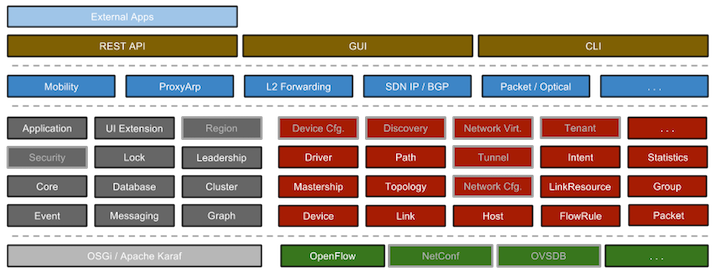
\includegraphics[width=1\textwidth]{ONOS_archi.png}
  	\caption{Architecture logicielle d'ONOS (schéma extrait du site officiel)}
\end{figure}

\begin{list}{$\Asteriscus$}{}

\item Au Sud : une API (southbound) gérant plusieurs protocoles (dont Openflow (toutes les versions jusqu’à la version 1.5, la version 1.6 étant en cours de prise en charge)). C’est la partie d’ONOS qui se charge de la communication avec les switchs. Il est ainsi possible de prendre en charge de nouveaux protocoles ou de nouveaux drivers.

\item Sur le côté : un protocole d’échange entre contrôleurs. Cela permet un contrôle partagé du réseau. Pour cela, des informations sur la topologie de celui-ci doivent être échangées entre contrôleurs. Le protocole en question n'est pas standardisé.

\item Au Nord : une API (northbound) permettant d’écrire des applications utilisant les ressources offertes par le contrôleur. Si le secure mode est activé (nous reviendrons plus en détail sur cela ultérieurement), l’ensemble des méthodes utilisables est restreint. 

\item Au Nord encore : une interface utilisateur fournie par Karaf et composée de 3 parties: une API REST accessible sur le port 8181 (configurable), une interface web (permettant de visualiser l’état du réseau, les applications lancées ...) accessible sur ce même port, et une CLI accessible en SSH sur le port 8101 (ou bien directement sur le contrôleur, là encore tout est configurable).

\end{list}
	\subsection{Surface d'attaque}
		Pour tester le contrôleur, l’installation suivante est actuellement réalisée :
- une machine virtuelle utilisant l'émulateur réseau mininet, qui crée des switchs et hôtes virtuels, et qui permet de générer du trafic réseau SDN.
- une machine virtuelle (ubuntu server) sur laquelle le contrôleur ONOS est installé et est accessible.
- une machine virtuelle (ubuntu desktop) permettant d’intéragir avec le contrôleur en SSH (on peut aussi utiliser la machine non virtuelle).

On va donc appliquer la méthode STRIDE aux divers éléments et interfaces qui composent ONOS, à la manière de ce qui est présenté dans un article de l'institut Fraunhofer \footnote{\url{http://publica.fraunhofer.de/eprints/urn_nbn_de_0011-n-4046948.pdf}}.

		\subsubsection{Menaces au niveau de l'interaction avec les switchs}
			Le contrôleur reçoit et interprète des données des switchs qu'il contrôle. Cela signifie que, si l'une des entités avec qui il communique est malveillante, celle-ci a la possibilité d'agir négativement sur le contrôleur.
En appliquant la méthode STRIDE à l'interface sud, on trouve 4 menaces :

\begin{itemize}

\item Usurpation d'identité (S) : possibilité pour un élement de se faire passer pour ce qu’il n’est pas (un switch se faisant passer pour un autre switch par exemple, ...).

\item Altération (T) : possibilité de modifier le flux de données des switchs en se plaçant sur le chemin du contrôleur (man in the middle). Cette partie est rapide à étudier puisque TLS, si il est correctement utilisé, permet d’éviter toute modification du flux.

\item Divulgation d'information (I) : possibilité d’obtenir les flux d’informations entre les éléments du réseau et le contrôleur (là encore si TLS est activé cela réduit la menace à son minimum).

\item Déni de service (D) : possibilité de surcharge des interfaces réseau, par exemple un switch non désiré sur le réseau qui surcharge le contrôleur de messages, de manière intelligente (en sachant ce qui ralentira le plus le contrôleur) ou non.

\end{itemize}

Dans la suite, on testera S, T, D (et pas I car on supposera TLS activé). Mais toujours relativement au contrôleur, c'est à dire qu'on regardera si le contrôleur agit comme il est supposé réagir, permettant ou non l'attaque. Et on constatera ou non la généricité des attaques.

		\subsubsection{Menaces au niveau de l'interaction utilisateur}
			Le contrôleur exécute potentiellement des applications fournies par des tiers. Si un utilisateur  importe une application malveillante sur le contrôleur, cela peut avoir des répercussions sur tout le réseau.
Concernant la méthode STRIDE appliquée à l'interface nord, on trouve majoritairement 5 menaces :

\begin{list}{$\Asteriscus$}{}

\item Spoofing (S) : (abus de langage ici, mais c'est la catégorie qui se rapproche le plus de la réalité) possibilité de modifier le comportement de certaines applications avec des droits non adaptés.

\item Tampering (T) : possibilité de modifier le flux de données des applications en se plaçant sur le chemin du contrôleur (man in the middle). Cette partie est rapide à étudier puisque là encore, TLS, si il est correctement utilisé, permet d’éviter toute modification du flux d'information.

\item Repudiation (R) : possibilité pour une application de nier certaines actions dont elle est l'origine.

\item Information disclosure (I) : possibilité d’obtenir des informations sur d'autres applications, sur l'état général du contrôleur, ...

\item Denial of service (D) : possibilité d'action néfaste sur le contrôleur (modification de la topologie, dégradation du débit offert par le contrôleur, ...).

\end{list}

Dans la suite, on testera S,T,D et I. Encore une fois cela sera fait par rapport à ONOS, ce qui ici se justifie d'avantage (aucun standard n'existant au niveau de l'interface nord, celle-ci peut varier beaucoup selon le contrôleur). De plus, ONOS propose un mécanisme de sécurité intéressant à étudier qui est le Security Mode, mis en place depuis la version Drake (1.3) du contrôleur.

\begin{figure}[h]
  	\centering
  	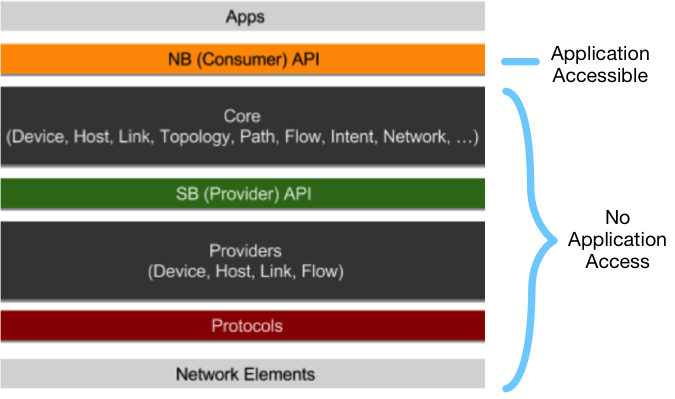
\includegraphics[width=0.6\textwidth]{secure_mode.png}
  	\caption{Secure mode activé : accès aux fonctions critiques restreint lors de l'utilisation de l'API par certaines applications}
\end{figure}

Ce module, qui continue d'être amélioré, rajoute la possibilité de définir des permissions fines (ce qui se traduit par le droit d'utiliser ou non certaines fonctions de l'API) par rôle aux applications, et sera légèrement détaillé plus tard. Les attaques qui constitueront cette partie seront donc moins génériques que les attaques menées au niveau de l'interface sud.

		\subsubsection{Autres menaces}
			Nous avons évoqué les menaces qui pesaient sur les interfaces nord et sud, mais il existe encore d'autres menaces :

\begin{itemize}

\item Sur le contrôleur en lui même : bien que cela soit laborieux et que je n'aie pas réussi à le faire durant mon stage, il n'est pas impossible qu'il existe des vulnérabilités dans le code source du contrôleur. Sans aller jusqu'à l'exécution de code arbitraire (sachant que le code est en Java, donc cela nécessite normalement une faille de la machine virtuelle, puisqu'à aucun endroit du code la possibilité est offerte d'exécuter du code externe si on supprime le cas d'une application externe), il est envisageable de trouver des enchaînements (mise à jour de variables bien choisies, modification de l'état interne du contrôleur) qui réalisent des actions non prévues. Cela demande cependant une connaissance excellente du code, ce qu'il est très compliqué d'obtenir vu le peu de documentation qui est offerte lorsqu'on souhaite se plonger dans le coeur du contrôleur et la complexité générale de l'ensemble.\\

Sur le contrôleur on peut aussi trouver un problème de répudiation : bien que les logs soient sauvegardés et soient assez complets, rien n'empêche à l'heure actuelle de les supprimer (le but étant plus de fournir du debug au développeur qu'un outil d'analyse forensique voire une preuve certaine des évènements passés).\\

Enfin toujours sur le contrôleur, on peut trouver des problèmes de DoS, comme par exemple en 2015 avec la CVE-2015-7516\footnote{https://wiki.onosproject.org/display/ONOS/Security+advisories}. Cela revient là encore à utiliser les faiblesses du code pour avoir une action non prévue néfaste sur les performances globales.\\

\item Sur les échanges inter-contrôleurs : le concept SDN prévoit la possibilité de gestion à plusieurs contrôleurs du réseau SDN. Pour cela, il est nécessaire que les contrôleurs partagent entre eux la topologie à laquelle ils ont accès. Cela introduit une vulnérabilité supplémentaire puisque sans authentification mutuelle, il existe un risque de parler à un contrôleur malveillant envoyant de fausses informations.\\

\item Sur les stations d'administration et de déploiement : comme sur un réseau classique, si on compromet les machines utilisées pour gérer le réseau ou distribuer les mises à jour logicielles (social engineering, compromission de l'environnement (DNS ou ARP spoofing, ...)), on a théoriquement un accès privilégié au contrôleur (selon les modes d'authentification utilisés) qui permet donc sans y être autorisé d'y apporter des modifications importantes.\\

\item Sur les éléments du réseau : bien que cela demeure peu probable, les mêmes attaques que sur un réseau classique sont toujours possibles. Elles permettent ensuite d'utiliser les attaques sur l'API southbound.

\end{itemize}

Le très récent site regroupant entre autres les projets Security-mode ONOS, Delta et Barista \footnote{http://sdnsecurity.org} (nous en reparlerons dans la conclusion) nous donne un bon récapitulatif d'une partie des attaques que nous allons détailler et qui s'inscrivent dans les catégories précédentes :
\begin{figure}[h]
  	\centering
  	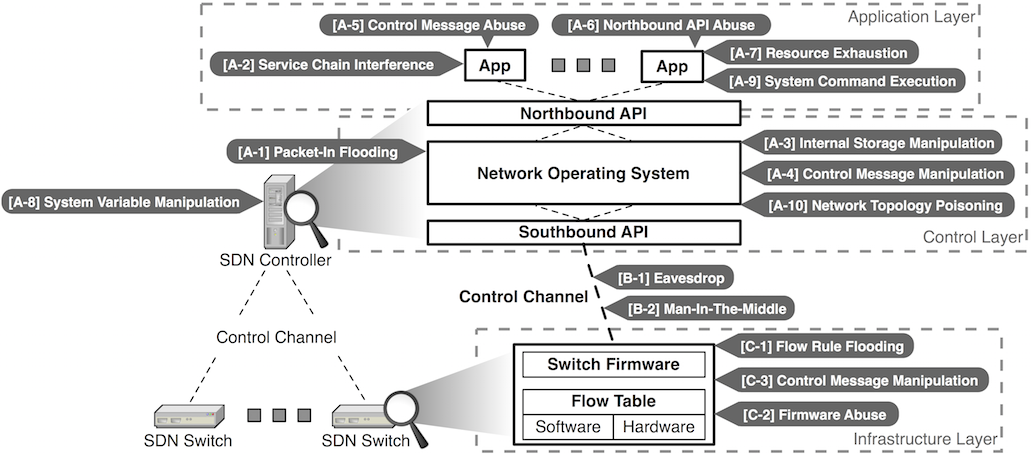
\includegraphics[width=1\textwidth]{threats.png}
  	\caption{Principales menaces sur un réseau SDN}
\end{figure}

	\subsection{Scénarios envisagés}
		Pour éclairer de manière expérimentale le large spectre de menaces auquel peut être soumis un réseau SDN, j'ai mis en place au fur et à mesure 6 preuves de concept, certaines n'étant pas très complexes mais démontrent toutefois certaines faiblesses. Même si parmi les scénarios envisagés il y en a certains qui sont spécifiques à ONOS (notamment ceux qui concernent l'interface nord), on verra que les attaques sont globalement les mêmes que dans un réseau classique, avec en revanche des impacts plus lourds.

Pour rester dans la nomenclature précédente, voici les attaques envisagées :

\begin{itemize}

\item \underline{Scénario 1 :} Tampering et Information disclosure (interface sud) \\
\underline{But :} Intercepter et modifier les communications sur le plan de données ou de contrôle si TLS n'est pas activé.

\item \underline{Scénario 2 :} Spoofing et DoS (interface sud) \\
\underline{But :} Altérer la topologie estimée par le contrôleur en usurpant l'identité d'un switch ou en inventant un faux switch et en créant des faux messages LLDP.

\item \underline{Scénario 3 :} DoS (interface sud) \\
\underline{But :} Réduire fortement le débit au niveau de certains nœuds par envoi d'un très grand nombre de paquets dont on espère qu'ils vont chacun aboutir à la création d'une règle au niveau du contrôleur. Ceci afin de surcharger les tables de flux des switchs visés.

\item \underline{Scénario 4 :} DoS (interface nord) \\
\underline{But :} Altérer les performances du contrôleur, tester certaines permissions critiques avec le Security Mode.

\item \underline{Scénario 5 :} Information disclosure (interface nord) \\
\underline{But :} A partir d'une application banale qui n'a pas le droit de regarder quelles sont les autres applications présentes sur le contrôleur, observer quels éléments peuvent quand même être rendus accessibles sans que cela soit explicitement prévu.

\item \underline{Scénario 6 :} Spoofing (interface nord) \\
\underline{But :} Tester la frontière entre permission liée à une application et permission liée à l'API REST.

\end{itemize}

Chacun de ces 6 scénarios est détaillé séparément dans la partie suivante.
\newpage
\fancyhead[L]{3- Audit}
\section{Audit}
	\subsection{Man in the middle au niveau de l'interface sud}
		\underline{Prérequis/Hypothèses :}\\
- Un switch malveillant connecté à un autre switch dans le réseau local\\
- Une machine A connectée directement à un switch s1 dans un sous réseau accessible depuis le switch malveillant\\
- Une machine B connectée indirectement à un switch s2\\
- A cherche à joindre B\\
- Le switch s1 a ses tables de flux par rapport au paquets ARP susceptibles d’être crées à partir de A vers B vides (c’est à dire aucune règle n’est susceptible d’appliquer une action prédéfinie aux paquets ARP provenant de A vers B (et donc génération d’un PACKET\_IN en conséquence)).
- Une topologie en partie connue (IP des hôtes à usurper) est un plus\\


\underline{Buts :}\\
- Tester la capacité du contrôleur à détecter des Man in the Middle, ce qui devrait s’avérer finalement plus simple que dans un réseau normal (en effet le contrôleur dispose normalement d’une vision globale de la topologie réseau à partir des switchs qu’il contrôle.

\underline{Déroulement :}\\
- La machine A cherche à contacter la machine B (ping par exemple)\\
- Une requête ARP est donc envoyée depuis A et s1 la retransmet au contrôleur n’ayant pas encore d’action associée au flux\\
- Le contrôleur renvoie le paquet en PACKET\_OUT sur le switch s1 qui le rediffuse\\
- Notre switch malveillant répond plus rapidement que l’équipement concerné à la requête ARP et cherche à intercepter la communication entre A et B voire à la supprimer

Dans la pratique, l'attaque se passe exactement comme dans un réseau classique : le switch malveillant envoie de très nombreuses fausses requêtes ARP en broadcast pour altérer les tables ARP des équipements cibles. On utilisera donc ettercap pour mener l'attaque.

\underline{Détails techniques :}\\
Se référer au scénario 1 décrit dans l'annexe (page).

\underline{Résultat :}\\
Comme sur un réseau classique, l'attaque fonctionne (on est à la fois en mesure d'intercepter et de modifier le trafic entre A et B). Cela s'explique facilement puisque les mécanismes utilisés pour le routage et le transport sont les mêmes. Si TLS n'est pas utilisé au sud on peut envisager l'attaque en plus sur le plan de contrôle, et donc pousser ses propres règles sur l'entité visée.

\underline{Parades proposées :}\\
Dans un réseau SDN, il me semble faisable de détecter et contrer ce genre d'attaque beaucoup plus facilement que dans un réseau classique. Si on enlève la solution TLS avec authentification mutuelle (qui permet de supprimer ce problème puisque le switch malveillant ne peux plus communiquer ni avec le contrôleur ni avec les autres switchs), on peut proposer 2 parades.

La première tient à la "signature" de l'attaque. Dans le cas d'une topologie inconnue par le switch malveillant, celui-ci va envoyer de nombreux paquets ARP pour découvrir les éléments présents sur le réseau. Or si aucune règle spéciale n'est présente sur les switchs, les paquets sont envoyés au contrôleur. Ce dernier peut donc détecter, si les envois sont trop rapprochés par exemple, une activité anormale en provenance d'une même adresse mac.

La seconde est encore liée à la capacité du contrôleur à disséquer les paquets qu'il reçoit. En effet, lors de l'attaque, il va recevoir des paquets ARP portant une adresse IP connue (la cible) associée à une adresse MAC ne correspondant pas à la description de l'hôte qu'il détient. Si il analyse les paquets ARP reçus, il peut donc détecter l'attaque. L'inconvénient de cette méthode est l'obligation de traiter chaque paquet ARP reçu, ce qui peut être éventuellement utilisé dans un but de DoS.

\underline{Limitations/Impact/probabilité :}\\
Comme sur un réseau traditionnel, l’attaque ne fonctionne qu’au sein d’un réseau local donc l’attaquant doit faire partie du réseau. De plus, même si les impacts de ce genre d’attaque peuvent être importants (la communication passant par une troisième entité, tout peut être modifié entre les équipements concernés) :\\
-d’une part l’utilisation d’un chiffrement entre contrôleur et switch permet théoriquement d’éviter à un élément non authentifié de faire partie du réseau (même si la gestion d’une PKI fiable au sein d’un réseau SDN est complexe à mettre en œuvre).\\
-d’autre part comme on l'a dit au dessus, le contrôleur SDN est mieux armé pour répondre à ce genre d’attaque qu’un réseau classique, au prix d'un surcoût éventuel en ressources (gestion de tous les paquets ARP depuis le contrôleur).
		\newpage
	\subsection{Altération de la topologie depuis l'interface sud}
		\underline{Prérequis/Hypothèses :}\\
- Une entité malveillante connectée au réseau local\\
- Une topologie en partie connue (adresse mac de deux switchs)\\
- 2 switchs s1 et s2 non reliés entre eux\\


\underline{Buts :}\\
L’hôte malveillant (en se faisant passer pour un switch) fait croire au contrôleur qu’il existe un lien entre lui et s1, ainsi qu’entre lui et s2. Si la manière dont ONOS calcule les plus courts chemins peut être exploitée et que l'hôte arrive à faire croire que ces liens sont rapides, il est possible que le contrôleur crée un nouveau lien logique entre s1 et s2. Cela engendre un déni de service puisque les paquets qui correspondront aux règles ajoutées sur les switchs s1 et s2 empruntant le faux lien seront envoyés à notre entité malveillante, pouvant les modifier ou tout simplement les détruire : on peut alors aboutir à un "trou noir" dans le réseau.

\underline{Déroulement :}\\
Notre hôte malveillant envoie de faux paquets LLDP en multicast pour simuler un lien entre lui, le switch s1 et le switch s2 (en utilisant le mécanisme de découverte de topologie d'ONOS évoqué à la page 15).

\underline{Détails techniques :}\\
Se référer au scénario 2 décrit dans l'annexe (page).

\underline{Résultat :}\\
L'attaque, en partie reproduite depuis l'article "Poisoning Network Visibility in Software-Defined Networks: New Attacks and Countermeasures" \footnote{\url{http://www.internetsociety.org/sites/default/files/10_4_2.pdf}}, fonctionne dans certains cas, permettant de stopper le contact entre s1 et s2. Je n'ai pas trouvé comment faire fonctionner l'attaque à chaque essai. Il est également envisageable d'intercepter/modifier du trafic réseau avec cette méthode même si je ne l'ai pas fait.

\underline{Parades proposées :}\\
Une solution intéressante proposée dans le document associé à l’attaque est de rajouter un champ dans les paquets LLDP envoyés par le contrôleur qui contienne une partie authentification : par exemple n’accepter des paquets LLDP que lorsqu’un champ supplémentaire crée par le contrôleur et basé sur certaines caractéristiques du switch auquel il est envoyé est vérifié (mécanisme de signature). Cela résiste à la fabrication de paquets sur un hôte, mais ne résiste pas si l’attaquant dispose d’un switch connecté au réseau qui est capable de recevoir des paquets LLDP. Toutefois, cela octroie une sécurité supplémentaire non négligeable puisqu’il devient impossible de mettre en œuvre cette attaque si on n’est pas physiquement connecté.

\underline{Limitations/Impact/probabilité :}\\
Là encore l’attaquant doit faire partie du réseau local. De plus, la détermination de la topologie (même supposée optimale) trouvée par le contrôleur n’est pas forcément simple à prévoir, et ce n’est pas dit que le faux lien qu’on indique sera effectivement utilisé par le contrôleur.\\
Donc encore une fois on a une attaque avec une probabilité (très) faible et un impact fort. On peut noter que l’avantage SDN précédent (obtenir beaucoup d'information locale pour construire une topologie globale) se retourne dans cette situation contre lui : vu que tout est centralisé, si on arrive à modifier la vision du réseau du contrôleur les conséquences sont plus graves contrairement à un réseau classique où il faudrait potentiellement modifier un grand nombre de routeurs avant d’arriver à un point de déni de service équivalent.
		\newpage
	\subsection{Deni de service au niveau de l'interface sud}
		\underline{Prérequis/Hypothèses :}\\
- Un switch malveillant connecté à un switch du réseau ou directement au contrôleur\\
- Une topologie en partie connue (adresse mac et IP des switchs à attaquer)\\


\underline{Buts :}\\
Surcharger les tables de flux d’un ou de plusieurs switch(s) pour provoquer un déni de service (moins de bande passante).

\underline{Déroulement :}\\
Notre switch malveillant peut envoyer à ses switchs voisins des paquets avec une adresse IP source, une adresse MAC source, un VLAN id, un type de service, un port TCP/UDP, aléatoires. Ainsi, les chances que le switch cible envoie un PACKET\_IN au contrôleur sont élevées. D’une part on consomme ainsi des ressources en envoyant beaucoup de PACKET\_IN, et d’autre part si les décisions prises par le contrôleur sont trop spécifiques (peu de jokers utilisés par exemple), le switch sur lequel seront appliquées les règles va progressivement se retrouver surchargé de règles inutiles.

\underline{Détails techniques :}\\
Se référer au scénario 3 décrit dans l'annexe (page).

\underline{Résultat :}\\
L’attaque est réussie : dans les conditions théoriques testées, on passe d’une bande passante de 6,7 Gb/s entre 2 hôtes, à une bande passante de quelques Mb/s (avec des pertes de paquets variables, mais pouvant s'élever jusqu'à un déni de service total). Parfois le déni de service est moins élevé et fournit des variations de débits importantes. Cela s'explique notamment par le fait que certaines règles souvent utilisées restent en haute priorité sur le switch malgré les tentatives de surcharge des tables de flux (et donc sont utilisées sur le plan de données avec des performances acceptables malgré les règles poubelles ajoutées).

\underline{Parades proposées :}\\
Les parades pour cette attaque sont assez nombreuses et relativement faciles à mettre en œuvre. Tout d’abord disposer au niveau du contrôleur d’algorithmes de création de règles capables d’agréger des flux (c'est à dire capacité de factoriser des règles avec des jokers). D’autre part une politique de filtrage générale a priori (par exemple DROP des paquets sur certaines IP/pour certains ports ou autre) s’avère très efficace (même si cela peut être pénalisant si on souhaite que par défaut les paquets inconnus puisse circuler facilement). En résumé, une politique réseau stricte conservant la flexibilité initiale avec des jokers dans les règles ajoutées aux tables de flux.

\underline{Limitations/Impact/probabilité :}\\
Pour cette troisième attaque, l’attaquant doit encore avoir un accès proche du réseau (il doit être connecté à un switch du réseau). De plus, si les switchs sont correctement configurés à la base (admettons que la politique du contrôleur soit une politique "opt-in" et non "opt-out", c’est à dire que par défaut les paquets ne sont pas transmis en PACKET\_IN au contrôleur mais jetés, sauf cas choisis par le contrôleur), alors l’attaque ne fonctionne plus. OpenFlow à partir de sa version 1.3 permet d’ailleurs à l’administrateur de définir les actions à appliquer à des paquets inconnus (auparavant ils étaient envoyés au contrôleur dans tous les cas). Les switchs sont normalement sensés pouvoir gérer un nombre suffisant de flux et de règles (cela est spécifié dans le premier OFPT\_FEATURES\_REPLY, par exemple avec les switchs virtuels mininet, ce paquet indique le support de 256 tables de flux). Le risque majeur de l’attaque est donc finalement l’écrasement de règles utiles par des règles qui ne le sont pas. Le risque est faible, l’impact moyen.
		\newpage
	\subsection{Deni de service au niveau de l'interface nord}
		\underline{Prérequis/Hypothèses :}\\
- Un éditeur d’application malveillant\\


\underline{Buts :}\\
Tester le secure mode d’ONOS. Regarder ce qu’il est possible d’effectuer comme action néfaste sur le contrôleur, sur les performances du réseau en général. Modifier la topologie du réseau, effacer les tables de flux.

\underline{Déroulement :}\\
Un utilisateur mal intentionné charge une application sur le contrôleur. Cette application contient des instructions de tous les types pour consommer les ressources du contrôleur et modifier son fonctionnement. Par exemple on testera si il est possible de provoquer l’arrêt du contrôleur. On testera également l’import et l’utilisation des fonctions de l’API d’ONOS bas niveau, c’est à dire celles qui sont susceptibles d’être utilisées par le coeur d’ONOS pour avoir des informations sur le réseau environnant. Enfin, on regardera si il est possible de monopoliser en partie certaines ressources du contrôleur (par exemple accès au disque, mais aussi processeur avec des calculs couteux répétés en boucle).

\underline{Détails techniques :}\\
Se référer au scénario 4 décrit dans l'annexe (page).

\underline{Résultat :}\\
Si le contrôleur n'est pas correctement configuré ou est volontairement permissif, il faut avoir une confiance absolue dans les applications qui tournent sans droits restreints. En effet, sinon il est possible d'effectuer toutes les actions envisageables sur le contrôleur et donc sur le réseau.

\underline{Parades proposées :}\\
Le secure mode a été mis en place pour parer ce genre de vulnérabilité, et il est efficace pour cela. C’est une protection cruciale qu’on est en droit d’attendre pour un tel contrôleur. Le secure mode est assez puissant car il offre un niveau de granularité très fin \footnote{\url{https://wiki.onosproject.org/display/ONOS/ONOS+Application+Permissions}}. Si l'administrateur général configure correctement le contrôleur et octroie à chaque fois le minimum de privilèges requis pour les applications dont il ne maitrise pas forcément l'origine, cela minimise le risque.

\underline{Limitations/Impact/probabilité :}\\
Cette fois la probabilité d’une telle attaque n’est pas à prendre à la légère. Compte tenu de l’offre des contrôleurs SDN concernant la possibilité d’ajouter facilement des applications au réseau, le risque de rencontrer un utilisateur malveillant désirant nuire au réseau ou seulement disposer de plus de ressources qu’allouées est élevé. L’impact d’une telle menace est élevé. Les vulnérabilités au sein du contrôleur même sont les plus dangereuses au sein d’un réseau SDN. C’est donc un point qu’il ne faut à aucun prix négliger lorsqu'on souhaite mettre en place un tel réseau. Encore une fois, si le contrôleur est compromis, tout l'est dans le domaine contrôlé.

		\newpage
	\subsection{Fuites d'information au niveau de l'interface nord}
		\underline{Prérequis/Hypothèses :}\\
- Un éditeur d’application malveillant\\


\underline{Buts :}\\
Voir quelles informations sensibles il est possible de collecter sur les autres applications tournant sur le contrôleur à partir d’une application malveillante. Avec le secure mode activé ou sans.

\underline{Déroulement :}\\
Un utilisateur écrit une application d’apparence quelconque mais cherche à utiliser ce qui est à sa disposition dans l’API d’ONOS pour d’une part obtenir des renseignements sur les applications tournant à côté de notre application malveillante, et d’autre part à modifier son fonctionnement, en altérant ce qu’elle est susceptible de recevoir. Lorsque le secure mode est activé, on vérifie que l’application n’a pas accès à des fonctions critiques, et on regarde quelles informations peuvent toutefois fuiter.

\underline{Détails techniques :}\\
Se référer au scénario 5 décrit dans l'annexe (page).

\underline{Résultat :}\\
Lorsque le secure mode n'est pas activé, ayant accès au service gérant les applications et aux services internes du contrôleur, on peut donc tout faire sur celles-ci (désactivation, envoi de données falsifiées, ...). Sinon, selon les permissions, on peut effectuer certaines actions qui ont plus ou moins d'impacts. Par exemple avec les droits d'accès en lecture au système de fichier, on peut lire certains bouts de mémoire du contrôleur et accéder à des informations pas forcément dénuées d'intérêt. Avec les droits d'accès aux informations des applications en lecture, on peut lister les applications présentes et obtenir d'autres informations.

\underline{Parades proposées :}\\
Si il est bien utilisé, le secure mode est efficace pour empêcher des fuites d'information non désirées. Là encore, la responsabilité de donner des droits corrects incombe à l'administrateur et ne doit pas être négligée. Si les permissions d'une application sont réduites au minimum, celle-ci n'a plus beaucoup de possibilités. Une autre protection envisageable permettant d'isoler chaque application des applications voisines est celle qui a été implémentée dans le contrôleur RoseMary (propriétaire), à savoir une séparation des droits d'accès à la mémoire du contrôleur en fonction de l'application (ainsi, contrairement à ONOS au sein duquel il est possible d'accéder à toute la mémoire utilisée par le contrôleur, RoseMary interdit à une application d'accéder à des pages mémoires dont elle n'est pas à l'origine).

\underline{Limitations/Impact/probabilité :}\\
Comme précédemment, le risque est élevé. Même si l’impact est plus faible que dans la situation précédente, si il est possible d’extraire de l’information de "vraies" applications, il est envisageable que cela puisse servir en vue d’une attaque ultérieure cette fois sur les vraies applications à un niveau plus haut (en ciblant par exemple des applications avec un niveau de privilège élevé). Cela demeure toutefois assez complexe à mettre en œuvre.

		\newpage
	\subsection{Mauvaise configuration au niveau de l'interface nord}
		\underline{Prérequis/Hypothèses :}\\
- Un contrôleur ONOS mal configuré (mot de passe faible pour l'API REST)\\
- Un utilisateur malveillant qui obtient en conséquence des droits d’utilisation de l’API Rest\\


\underline{Buts :}\\
Tirer parti de la politique de gestion d’accès en mode role-based pour qu’un utilisateur avec des droits suffisants puisse altérer de manière non prévue le fonctionnement du contrôleur ou de certaines applications.

\underline{Déroulement :}\\
Un utilisateur mal intentionné utilise des fonctionnalités de l’API Rest d’ONOS pour modifier le plus possible le bon fonctionnement du contrôleur.

\underline{Détails techniques :}\\
Se référer au scénario 6 décrit dans l'annexe (page).

\underline{Résultat :}\\
Depuis l'API REST il est possible d'avoir un impact conséquent sur toutes les parties du contrôleur (applications, mais aussi éléments du réseau et configuration interne). On peut par exemple choisir le comportement par défaut associé à la réception d'un PACKET\_IN depuis l'API (et donc éventuellement court-circuiter la réception du paquet par des applications quelconques si on choisit de tout renvoyer automatiquement en tant que PACKET\_OUT \footnote{\label{ONOS_REST}http://nss.kaist.ac.kr/wp-content/uploads/2016/05/p23-lee.compressed.pdf}), désactiver ou activer une application, supprimer un élément réseau connecté ...

\underline{Parades proposées :}\\
Le fait de mélanger des droits utilisateurs (au niveau de l'API REST) et des droits pour chaque application (au niveau du Security Mode) est relativement gênant dans la mesure où un utilisateur avec des droits suffisants peut théoriquement agir sur toutes les applications existantes sans distinction. Il faudrait je pense ajouter la possibilité de pouvoir agir uniquement sur certaines applications (créer des groupes d’applications qu’on associe à un droit particulier, de cette manière un utilisateur peut avoir les droits de modifications sur certaines applications et pas sur d’autres). Mais là encore, si l'administrateur configure les permissions de manière correcte et si peu de gens ont un accès à l'API REST d'administration, cela constitue une bonne première défense.

\underline{Limitations/Impact/probabilité :}\\
L’impact de cette "attaque" est fort (la modification de certaines options peut entraîner de nombreux DoS potentiels). La probabilité elle, reste faible, car l’utilisateur malveillant doit tout de même disposer des droits liés à l’utilisation de l’API ainsi que d’un accès à l’API. Il faut donc veiller à changer les identifiants par défaut sur l’interface nord pour éviter qu’un utilisateur quelconque puisse utiliser cette API et prévoir une politique de gestion de mot de passe robuste à ce niveau.
\newpage
\fancyhead[L]{4- Evaluation et recommandations}
\section{Validation et évaluation}
	\subsection{Résultats de l'étude}
		6 attaques ont donc été réalisées et s'avèrent fonctionnelles (même si les impacts et risques pour chacune sont assez différents). Dans les différentes conclusions tirées, on trouve principalement deux éléments communs :

\begin{itemize}

\item La possibilité de contrer certaines attaques lorsqu'on rajoute des modules au contrôleur (algorithmes factorisant la création de règles, gestion des paquets ARP par le contrôleur ...). Cela nécessite cependant du temps (de développement) et peut s'avérer coûteux au niveau du temps de traitement sur le contrôleur.

\item La nécessité de configurer correctement ONOS au niveau de l'interface nord, et d'être conscient de l'implication éventuelle de chaque permission octroyée en terme de potentiel d'action sur le contrôleur. Cela étant primordial pour éviter la prise de contrôle du contrôleur par une entité externe.

\end{itemize}

Les trois premières attaques permettent de montrer qu'on retrouve les vulnérabilités de réseaux classiques sur un réseau SDN. Les impacts y sont globalement plus élevés mais les contre-mesures plus simple à prendre (avoir une vue globale du réseau permet rapidement de bien estimer l'impact d'une action quelconque, ce qui n'est pas forcément réalisé sur un réseau décentralisé).
Les trois dernières sont propres à ONOS mais on retrouve les mêmes problématiques sur tous les contrôleurs SDN. ONOS et OpenDayLight restent à ma connaissance les contrôleurs les plus avancés en matière de sécurité, grâce aux modes additionnels qu'ils proposent (Security Mode pour ONOS et AAA (Authentification-Authorization-Accounting) pour OpenDayLight). OpenDayLight implémente même un module anti DoS. On trouve ainsi un certain nombre de documents qui attestent la dangerosité liée à la possibilité d'installation d'applications externes non vérifiées sur des contrôleurs qui ne disposent pas toujours de mécanismes de protection avancés.

Les tests effectués sont cependant loin de couvrir l'intégralité des menaces qui existent sur le contrôleur, c'est pourquoi la partie suivante tente de compléter celles-ci.

	\subsection{Autres considérations}
		Je ne l'ai découvert que trop tard, mais durant la blackhat 2016, s'est déroulée une présentation sur le sujet du stage \footnote{\url{https://www.blackhat.com/docs/us-16/materials/us-16-Yoon-Attacking-SDN-Infrastructure-Are-We-Ready-For-The-Next-Gen-Networking.pdf}}. Cette présentation résume les différents points névralgiques d'ONOS et d'OpenDayLight, et les schémas y sont limpides (pour les lecteurs désirant bien se figurer certaines attaques). 

Parmi les principales attaques qui n'ont pas encore été évoquées, on trouve :

\begin{list}{$\Asteriscus$}{}

\item les attaques sur les switchs : si ceux-ci n'implémentent pas correctement le protocole Openflow ou sont faiblement configurés et qu'il est possible d'en prendre le contrôle, on se retrouve dans le cas où on peut plus facilement exécuter les attaques précédentes sur l'interface sud d'homme au milieu et de deni de service.

\item les attaques liées à la gestion multi-contrôleurs éventuelle : il existe une possibilité de contrôler un switch depuis plusieurs contrôleurs à la fois (par exemple pour assurer le service si un contrôleur tombe en panne) et également une possibilité d'échange d'informations entre contrôleurs. Or il n'existe pas encore ni de mécanisme standardisé ni de sécurité très élevée pour de tels échanges, et la capacité des switchs à être contrôlés par plusieurs contrôleurs repose sur la notion de contrôleurs maître/esclaves qui peut aboutir à un deni de service si un contrôleur malveillant monopolise le rôle de maître sur un switch (sans parler des vulnérabilités existantes sur les switchs qui permettent même en étant un contrôleur esclave de modifier les tables de flux \footnote{Un collègue à Telecom Sudparis a travaillé sur ce point et montré la vulnérabilité sur certains switchs}).

\item les attaques sur le plan de communication : comme on l'a déjà dit, sans TLS, pas de confidentialité ni de confiance dans les données qui transitent via Openflow et donc possibilité pour un attaquant situé dans le réseau de prendre le contrôle d'une partie de celui-ci et de créer des messages malicieux dirigés contre le contrôleur. Mais l'activation de TLS avec authentification mutuelle n'est pas évidente à mettre en place (PKI fiable, qui puisse assurer la révocation, ...).

\item les attaques sur les environnements de développement et de déploiement : lors de la construction du contrôleur avec maven le code mais aussi d'autres éléments nécessaires peuvent être (et le sont même dans tous les cas réels) obtenus de manière distante sur des dépôts externes. Si la machine utilisée est corrompue (fichiers de configurations modifiés, DNS cache poisoning, ARP spoofing, malware, ...) alors toute l'installation qui en découle sur les contrôleurs peut fournir une opportunité énorme à l'attaquant de contrôler l'ensemble du réseau. C'est une menace très importante en terme d'impact et dont la probabilité n'est pas si faible qu'on pourrait le penser (social engineering, concentration des efforts sur une seule cible).

\item les attaques sur les stations de contrôle et d'administration : vu que certains éléments du conteneur OSGi d'ONOS permettent d'obtenir des droits importants sur le réseau, il est, comme sur un réseau classique, crucial de bien protéger les machines utilisées pour l'administration (là encore le social engineering peut être utilisé).

\end{list}

Pour bien mettre en valeur les spécificités éventuelles d'ONOS, le tableau suivant récapitule impacts et parades des différentes catégories d'attaque qu'on est susceptible de retrouver.

\begin{small}

\begin{tabularx}{\textwidth}{|X|X|X|}

\hline
Catégorie\newline d'attaque et spécificité & Impact & Parade\\
\hline
Flux réseaux forgés \newline -non spécifique SDN \newline -non spécifique ONOS & Injection de trafic pouvant conduire à du DoS ou de l'homme au milieu avec des conséquences plus grandes que sur un réseau classique & Programmation intelligente du contrôleur\\ 
\hline 

\end{tabularx}

\end{small}
	\subsection{Retour sur la méthode STRIDE}
		Comme l'audit a été fait en suivant partiellement la méthode STRIDE, et bien que le tableau du paragraphe précédent soit important à suivre, on va formuler la conclusion de l'étude sous la forme de la matrice habituellement utilisée avec cette méthode (différents éléments du système à gauche, différents risques en haut du tableau).\\
Parmi les éléments du système, on trouve :\\
- le processus principal (coeur du contrôleur)\\
- les flux de données (deux au niveau de l'interface nord (gestion, et applications), un autre au niveau de l'interface sud)\\
- les entités en interaction avec le contrôleur (switchs, applications, et machines d'administration)

\begin{small}

\begin{tabular}{|c|c|c|c|c|c|c|c|} 
    
\hline
Type & Composant & \textbf{S} & \textbf{T} & \textbf{R} & \textbf{I} & \textbf{D} & \textbf{E} \\
\hline
Processus & Coeur du contrôleur &  \circled{-} & \circled{-} & \circledgreen{1} & \circledcyan{2} & \circledorange{3} & \circledcyan{2}\\
\hline
 & Interface nord (gestion) &  & \circledcyan{4} &  & \circledcyan{4} & & \\
Flux de données & Interface nord (applications) &  & \circledcyan{4} &  & \circledcyan{4} & \circled{-} & \\
 & Interface sud &  & \circledcyan{4} &  & \circledcyan{4} & \circledred{5} & \\
\hline
& Machines d'administration & \circledcyan{6} &  & \circledorange{1} &  &  &  \\
Entités en interaction & Applications & \circled{-} &  & \circledorange{1} &  &  &  \\
& Switchs & \circledorange{7} &  & \circledgreen{1} &  &  &  \\
\hline
\end{tabular}
\begin{figure}[h]
\caption{Matrice STRIDE appliquée au contrôleur}
\end{figure}

\circledgreen{X} : mécanismes de protection déjà existants et activés par défaut\\
\circledcyan{X} : mécanismes de protection déjà existants mais à activer\\
\circledorange{X} : mécanismes de protection incomplets ou incertains\\
\circledred{X} : mécanismes de protection non existants\\
\circled{-} : mécanisme de protection inconnu ou ne pouvant pas être défini

\end{small}

Pour compléter le tableau précédent, voici les explications des chiffres :
\begin{list}{$\Asteriscus$}{}
\item 1 : Si le coeur d'ONOS est intègre, les logs sont enregistrés en permanence sur le disque par défaut ce qui permet à la fois le debug d'application et la tracabilité des connexions et évènements réseau divers. Cependant, mettre en place un système de sauvegarde distant ou empêcher une application avec des droits d'écriture de réécrire le fichier de log n'est pas aisé.
\item 2 : Le Secure-Mode permet à la fois d'empêcher des applications un peu trop curieuses d'accéder à ce qu'elles n'ont pas le droit d'accéder et d'exécuter des actions qu'elles ne sont pas sensées faire. Encore faut-il l'activer.
\item 3 : ONOS génère de nombreuses exceptions au cours de son fonctionnement, et toutes ces exceptions sont sauvegardées, générant une trace énorme et consommant une certaine quantité de ressources. Il n'est pas impossible de créer une application qui exploite cela. Il existait d'ailleurs une vulnérabilité importante (CVE-2015-7516\footnote{https://wiki.onosproject.org/display/ONOS/Security+advisories}) sur la version 1.3 du contrôleur qui provoquait la déconnexion de switchs lors du non traitement d'une exception.
\item 4 : L'utilisation de TLS, inactivé par défaut, permet de solutionner les problèmes de fuites d'informations et de modifications non souhaitées du flux au niveau des interfaces nord et sud (modulo la sûreté du protocole, comme toujours).
\item 5 : Le protocole Openflow n'a pas été conçu pour empêcher le deni de service, donc il est possible d'utiliser certaines parties de la spécification pour provoquer ce type d'attaque (voir les deux dernières attaques de l'audit sur l'interface sud).
\item 6 : L'usurpation d'identité d'un administrateur peut se faire si la configuration de l'authentification au niveau du contrôleur (GUI, CLI, ssh) est celle par défaut. Il ne faut pas oublier de changer les identifiants, ou de désactiver les services qu'on ne souhaite pas utiliser.
\item 7 : La deuxième attaque réalisée prouve qu'ONOS ne gère pas d'authentification pour les entités réseau au sud, ce qui permet l'usurpation d'identité de switchs. Cependant il existe maintenant une application en cours de développement (AAA, comme sur OpenDayLight) qui permet de corriger en partie le problème\footnote{https://wiki.onosproject.org/pages/viewpage.action?pageId=6357336}.
\end{list}
	\newpage
	\subsection{Conclusion}
		Comme on peut le constater, la route est encore longue avant de pouvoir disposer d'un contrôleur complètement fiable et imprenable, et de moyens permettant de vérifier cette fiabilité.

Le paradigme SDN est de toute façon, par nature, soumis à des menaces plus importantes. En effet, toute abstraction simplifiant ce sur quoi elle repose, permet avec beaucoup moins d'efforts d'obtenir un résultat équivalent (pensons aux systèmes d'exploitation actuels et à quel point ils nous simplifient la vie de manière considérable en abstrayant les instructions machines). Le même raisonnement peut s'appliquer ici : on peut s'attendre à ce que la gestion du réseau soit beaucoup plus agréable et simple avec l'adoption de SDN, mais cela repose sur 2 choses :

\begin{list}{$\Asteriscus$}{}

\item le système d'exploitation réseau doit être fiable (on vient de le voir, c'est très difficile à obtenir, car les menaces sont nombreuses et distantes. Si on revient à la comparaison avec les systèmes d'exploitation au sens classique, certes il est relativement "simple" de compromettre une machine lorsqu'on y a un accès physique, mais ça l'est beaucoup moins en cas d'accès distant. Or avec un système d'exploitation réseau tout n'est qu'accès distant, donc l'accès aux primitives de base du système est plus simple que sur un PC (plus simple de s'immiscer sur un réseau pour y envoyer une instruction Openflow que de s'immiscer sur un PC pour y exécuter une instruction assembleur)). Si des efforts suffisants sont déployés, il est envisageable d'obtenir ce point, mais cela demande une visions globale et une vigilance très importante sur ce qui est déployé sur le contrôleur. Dans l'idéal on peut supprimer un risque important en interdisant le déploiement d'applications qui n'ont pas été scrupuleusement vérifiées sur le contrôleur.
\item le système d'exploitation réseau doit être performant. Certes l'exemple de google montre qu'il est possible d'utiliser quasiment 100\% des liens, mais la présence du contrôleur et la nécessité de rediriger certains paquets vers lui peut ralentir le débit global. De plus on ne dispose pas encore de données sur les performances réelles obtenues en production (ce qui est dommage puisque cela ne pousse pas l'industrie frileuse à envisager une adoption progressive de SDN).

\end{list}

Si ces deux points réunis, il n'y a pas de raison pour que le déploiement de SDN ne se poursuive pas en dehors des gros data centers (mais cela reste un avis personnel uniquement basé sur une logique qui ne prend pas trop en compte la façon dont les réseaux actuels se déploient réellement). ONOS, pour l'avoir étudié d'avantage en détail, me semble un contrôleur prometteur (mais est assez proche d'OpenDayLight dans la structure et la philosophie, donc il est assez difficile de se prononcer sur un éventuel contrôleur représentant SDN qui soit beaucoup plus avancé que ses concurrents). Même si certains contrôleurs comme RoseMary ou SE-floodlight proposent des protections supplémentaires notamment concernant la mémoire bien isolée pour chaque application, la possibilité de distribution d'ONOS (et d'OpenDayLight d'ailleurs) et sa grande extensibilité lui confère un potentiel de déploiement industriel intéressant. 

Bien que l'ordre des opérations indiqué soit assez subjectif, on pourra si on souhaite déployer un réseau SDN avec le contrôleur ONOS vérifier dans l'ordre les points suivants :\\
- Déployer le contrôleur sur un réseau privé\\
- Séparer le réseau privé de gestion et le réseau privé de commutation\\
- Sécuriser le conteneur OSGi (donc ici Apache-Karaf), c'est à dire changer tous les identifiants par défaut\\
- Sécuriser les éventuels bundle OSGi rajoutés (permissions les plus basses pour tout nouveau bundle par défaut notamment)\\
- Changer tous les identifiants par défaut\\
-
\newpage
\fancyhead[L]{5- Conclusion}
\section{Perspectives à l'issue du stage}
	A l'issue de ce stage, après avoir successivement découvert le paradigme Software Defined Networking, évalué sa sécurité sur la base de ce qui avait déjà été publié sur le sujet et testé des attaques plus ou moins réalistes contre ce genre de réseau, je me suis convaincu, en partie irrationnellement (puisqu'il n'existe pas vraiment de cas d'école démontrant sur la base de mesures réelles la supériorité ou non de SDN en termes de performance) que les réseaux futurs seraient au minimum en partie des réseaux de ce type.\\
Si la sécurité complète de ces réseaux semble impossible à obtenir, puisqu'une entité reste toujours aussi faible que son point le plus faible et qu'il existe de nombreux points d'entrée sur un réseau SDN, il est nécessaire que ce soit l'une des composantes principales sur laquelle se base la construction ou l'amélioration d'un contrôleur.\\
Déployé localement et sur des réseaux isolés, les éventuelles faiblesses du paradigme peuvent ne pas s'avérer trop problèmatiques pour un administrateur conscient des risques encourus, surtout au regard des améliorations apportées en terme de flexibilité.\\
L'implantation durable de cette technologie n'est pas encore claire mais il semblerait que la tendance des investissements dans le domaine soit à une hausse significative depuis 2015 et continue de l'être. Même si la technologie n'est pas encore complètement mature, et que la spécification Openflow évolue très rapidement avec une complexité croissante (forçant une compatibilité partielle et des spécifications parfois mal appliquées au niveau des switchs), le nombre de projets et de tests semble proliférer. Certes la mise en production généralisée n'est pas pour tout de suite, mais de mon point de vue les avantages théoriques du software defined network surpassent ses inconvénients. L'important étant de rester conscient des nombreuses faiblesses d'une telle solution.\\

Aussi, c'est une ouverture optimiste que je formule : même si SDN n'est pas encore prêt pour la gestion de réseaux critiques, l'utilisation de l'ensemble contrôleur Openflow + switchs compatibles + Openflow permet de remplacer de nombreux protocoles propriétaires ou trop lourds tout en fournissant une vue détaillée et globale de l'état du réseau ainsi qu'un moyen d'appliquer facilement des politiques réseau complexes. C'est pourquoi il conviendrait à mon sens d'accompagner la transition vers ce type de réseau en fournissant petit à petit des moyens de consolidation, d'évaluation et de certification, de contrôleurs comme de switchs, principalement concernant leur sécurité. Pour en revenir une dernière fois avec l'analogie du système d'exploitation classique : qui s'imaginerait encore aujourd'hui coder en assembleur des pièces logicielles de plus en plus complexes ? Si on s'imagine assez mal à quoi pourraient ressembler des pièces logicielles réseau de plus en plus complexes, c'est peut être aussi parce qu'on a toujours considéré le réseau non pas comme quelque chose qui s'adapte en permanence à son environnement en fournissant un service dynamique, mais comme un élément statique servant uniquement à transporter de l'information d'un endroit à un autre. Il est peut être temps de changer d'approche ! (Cependant il ne faut pas se laisser distraire par les mots et les analogies, seule la réalité et les expériences de déploiement à large échelle pourront confirmer ou non les qualités supposées du SDN).\\

D’un point de vue personnel, je suis très satisfait d'avoir pu découvrir ce sujet dont je ne connaissais pas l'acronyme au départ, le tout au sein d'une équipe de recherche très conviviale. J'ai donc aussi pu me familiariser avec le monde de la recherche, ses avantages (liberté intellectuelle énorme, organisation libre, ...) et ses inconvénients (buter longtemps et en partie seul sur certains problèmes pas forcément intéressants, ne pas savoir où aller parfois). Encore une fois, SDN trace la voie des réseaux du futur, mais fournit un travail conséquent aux développeurs pour que le concept puisse devenir une perspective commerciale sécurisée et performante.

\newpage
\fancyhead[L]{6- Ressources}
\begin{small}
\bibliographystyle{plain}
\bibliography{references.bib}
\end{small}
\nocite{*}

\newpage
\fancyhead[L]{~\\}
\appendix
\section{Annexe}
	Cette partie montre comment mettre en place tous les éléments pour reproduire les attaques évoquées précédemment. On commencera donc par installer ONOS, mininet, puis on téléchargera certains outils pour reproduire les attaques.

\subsection{Installation d'ONOS}

Choisir une machine (virtuelle ou non) sur laquelle installer le contrôleur (durant le stage j'ai utilisé une debian serveur avec accès ssh pour y mettre ONOS). Sur la machine, installer java8 si il ne l'est pas encore. Cloner le dépôt des sources du contrôleur à l'adresse \url{https://gerrit.onosproject.org/onos}. Cloner également le dépôt git à l'adresse \url{https://github.com/Alkanoor/ONOS-Attack.git}. Télécharger apache-karaf et maven.

\begin{minted}{bash}
$ git clone https://gerrit.onosproject.org/onos
$ git clone https://github.com/Alkanoor/ONOS-Attack.git
$ mkdir Downloads Applications
$ cd Downloads
$ wget http://archive.apache.org/dist/karaf/3.0.5/apache-karaf-3.0.5.tar.gz
$ wget http://archive.apache.org/dist/maven/maven-3/3.3.9/binaries/apache-maven -3.3.9-bin.tar.gz
$ tar -zxvf apache-karaf-3.0.5.tar.gz -C ../Applications/
$ tar -zxvf apache-maven-3.3.9-bin.tar.gz -C ../Applications/
$ cd ..
\end{minted}

\subsection{Installation de Mininet}

Il est possible de suivre les instructions à l'adresse \url{http://mininet.org/download/}. Télécharger l'image qui convient la plus récente sur github (actuellement 2.2.1) : \url{https://github.com/mininet/mininet/wiki/Mininet-VM-Images}. La machine virtuelle offre un accès ssh avec les identifiants \textit{mininet / mininet}.

Il est également possible d'installer mininet sur une machine virtuelle déjà existante en clonant \url{git://github.com/mininet/mininet} et en exécutant \textit{mininet/util/install.sh} dans le dossier mininet.

Sur la machine virtuelle utilisée (si ça n'est pas la même que celle contenant ONOS), cloner également le dépôt \url{https://github.com/Alkanoor/ONOS-Attack.git}

\subsection{Configuration}

Pour que les attaques soient faciles à exécuter, les identifiants par défaut ne seront pas changés. Par contre il faut évidemment que la machine virtuelle contenant ONOS et celle contenant Mininet soient sur un même sous réseau.

Après avoir cloné le dépôt contenant les attaques sur les 2 machines, on va faire un test basique pour vérifier que tout fonctionne. Pour commencer on va configurer rapidement ONOS. Tout d'abord il faut éditer le fichier \textit{org.apache.karaf.features.cfg} en ajoutant mvn:org.onosproject/onos-features/1.9.0-SNAP-SHOT/xml/features (avec une virgule pour séparer le nouvel élément des attributs déjà présents) au niveau de la ligne "featuresRepositories" du fichier.

\begin{minted}{bash}
$ nano $(pwd)/Applications/apache-karaf-3.0.5/etc/org.apache.karaf.features.cfg
$ #modifier la ligne featuresRepositories en y ajoutant mvn:org.onosproject/onos-
$ #features/1.9.0-SNAPSHOT/xml/features
\end{minted}

Pour cela, on édite le fichier \textit{onos/tools/dev/bash\_profile} et on le charge dans le .bashrc (cela permet de bien mettre à jour l'environnement). Utiliser maven une première fois pour remplir le fichier profile.

\begin{minted}{bash}
$ echo '#ONOS environment'>>~/.bashrc
$ echo . $(pwd)/onos/tools/dev/bash_profile>>~/.bashrc
$ cd onos
$ mvn clean
\end{minted}

Pour changer les identifiants par défaut (\textit{grep \$(pwd)/onos/tools/dev/bash\_profile -e "ONOS"} changer les variables ONOS\_USER et ONOS\_GROUP avec le nom de l'utilisateur actuel, et éventuellement les variables ONOS\_WEB\_USER, ONOS\_WEB\_PASS (identifiants pour l'interface web)).
Quitter le shell en cours pour charger le nouveau .bashrc (ou le charger directement avec source).
Puis compiler ONOS (ceci prend un certain temps (au minimum une quinzaine de minutes)).

\begin{minted}{bash}
$ mvn clean install
\end{minted}

Lancer ONOS avec
\begin{minted}{bash}
$ ok clean #onos-karaf clean
\end{minted}


\end{document}